

\chapter{Bausteinsicht}

Um ein besseres Verständnis über die Struktur des Systems zu bekommen, nutzen wir die Bausteinsicht. Sie hilft dabei ein gemeinsames Verständnis des Systems innerhalb des Teams zu bekommen.
Die zur Zerlegung benutzte Dekompistionsstrategie ist funktional. 

\section{Bausteinsicht Level 1}
 

\begin{figure}[ht] % [h] = here
    \centering
    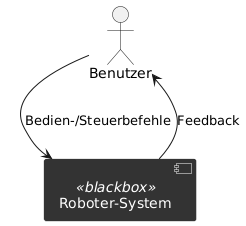
\includegraphics[width=0.6\textwidth]{diagrams/baustein_lvl_1_updated.png}
    \caption{Bausteinsicht Level 1}
\end{figure}

\begin{table}[h!]
\centering
\begin{tabular}{|p{4cm}|p{9cm}|}
\hline
\textbf{Komponente} & \textbf{Beschreibung} \\ \hline
Roboter-System & Gesamtsystem, das alle internen Steuer-, Safety- und Kommunikations­funktionen kapselt. Empfängt Bedien-/Steuerbefehle vom Benutzer, verarbeitet sie und liefert Feedback. \\ \hline
\end{tabular}
\caption{Bausteinsicht Level 1}
\label{tab:lvl1}
\end{table}

\newpage
\section{Bausteinsicht Level 2}
\begin{figure}[h] % [h] = here
    \centering
    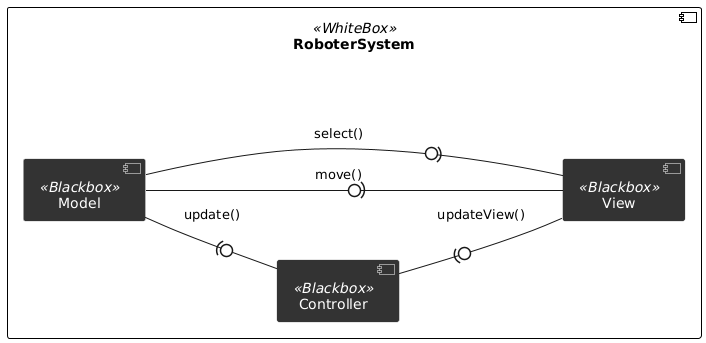
\includegraphics[width=0.6\textwidth]{diagrams/baustein_lvl_2_updated.png}
    \caption{Bausteinsicht Level 2}
\end{figure}

\begin{table}[h!]
\centering
\begin{tabular}{|p{4cm}|p{9cm}|}
\hline
\textbf{Komponente} & \textbf{Beschreibung} \\ \hline
Model & Beinhaltet die Geschäftslogik. Sendet periodisch Zustandsinformationen an den Controller. \\ \hline
Controller &  Der Controller leitet die Informationen vom StateService an die View weiter. \\ \hline
View & Bietet Interaktionsmöglichkeiten für den Nutzer und stellt dem Benutzer Informationen dar. 
\end{tabular}
\caption{Bausteinsicht Level 2}
\label{tab:lvl2}
\end{table}
\newpage

\section{Bausteinsicht Level 3 Model}
\begin{figure}[h] % [h] = here
    \centering
    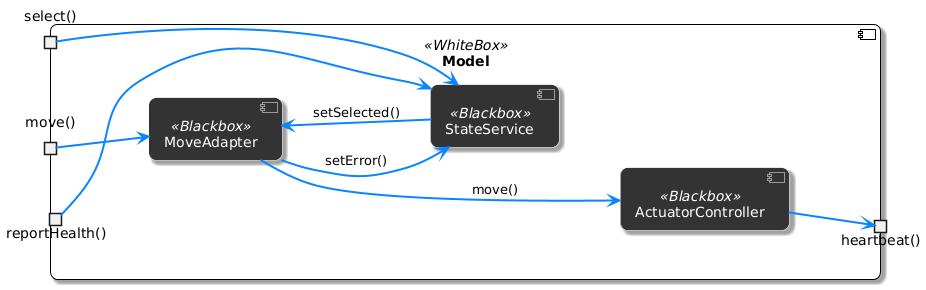
\includegraphics[width=0.6\textwidth]{diagrams/baustein_lvl_3_model_updated.png}
    \caption{Bausteinsicht Level 3 Model}
\end{figure}

\begin{table}[h!]
\centering
\begin{tabular}{|p{4cm}|p{9cm}|}
\hline
\textbf{Komponente} & \textbf{Beschreibung} \\ \hline
StateService & Speichert die Zustandsänderungen, informiert periodisch den Controller. 
Informiert den MoveAdapter über den derzeitigen selektierten Roboterarm. Durch die reporthealth() Methode, werden die Zustände der verschiedenen Aktoren überwacht. Darauf aufbauend wird die Liste der verfügbaren Roboter aufgebaut.\\ \hline
MoveAdapter  & Empfängt einen Steuerungsbefehl vom View, übersetzt diesen um den passenden Aktuator anzusprechen. \\ \hline
ActuatorController & Empfängt einen Steuerwert, überprüft die Gültigkeit und setzt diesen mithilfe der ICadsRoboticArm API. Sendet einen heartbeat an den Watchdog. \\ \hline
\end{tabular}
\caption{Bausteinsicht Level 3}
\label{tab:lvl3}
\end{table}

\section{Bausteinsicht Level 3 View}
\begin{figure}[h] % [h] = here
    \centering
    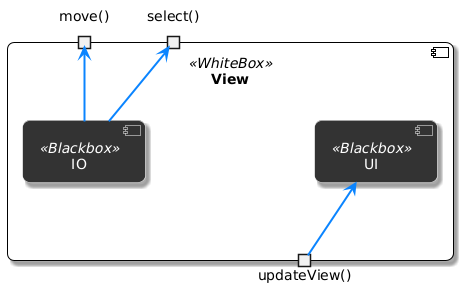
\includegraphics[width=0.6\textwidth]{diagrams/baustein_lvl_3_view_final.png}
    \caption{Bausteinsicht Level 3 View}
\end{figure}

\begin{table}[h!]
\centering
\begin{tabular}{|p{4cm}|p{9cm}|}
\hline
\textbf{Komponente} & \textbf{Beschreibung} \\ \hline
IO & Leitet die Steuerungsbefehle des Benutzers an den MoveAdapter weiter. Leitet Selektierungsbefehle an den StateService. \\ \hline
UI  & Stellt dem Nutzer dar welche Roboter verfügbar sind, welcher ausgewählt ist und gibt Rückmeldungen (Fehler, Bestätigungen).\\ \hline
\end{tabular}
\caption{Bausteinsicht Level 3: View}
\label{tab:lvl3}
\end{table}

\section{Bausteinsicht Level 3 Controller}
\begin{figure}[h] % [h] = here
    \centering
    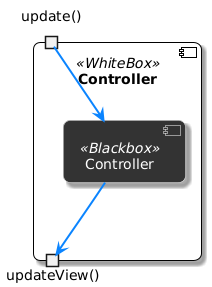
\includegraphics[width=0.6\textwidth]{diagrams/baustein_lvl_3_controller_final.png}
    \caption{Bausteinsicht Level 3 Controller}
\end{figure}

\begin{table}[h!]
\centering
\begin{tabular}{|p{4cm}|p{9cm}|}
\hline
\textbf{Komponente} & \textbf{Beschreibung} \\ \hline
Controller & Leitet Nachrichten des StateService an das View weiter. \\ \hline 
\end{tabular}
\caption{Bausteinsicht Level 3: Controller}
\label{tab:lvl3}
\end{table}



